% Options for packages loaded elsewhere
\PassOptionsToPackage{unicode}{hyperref}
\PassOptionsToPackage{hyphens}{url}
\PassOptionsToPackage{dvipsnames,svgnames,x11names}{xcolor}
%
\documentclass[
  letterpaper,
  DIV=11,
  numbers=noendperiod]{scrartcl}

\usepackage{amsmath,amssymb}
\usepackage{iftex}
\ifPDFTeX
  \usepackage[T1]{fontenc}
  \usepackage[utf8]{inputenc}
  \usepackage{textcomp} % provide euro and other symbols
\else % if luatex or xetex
  \usepackage{unicode-math}
  \defaultfontfeatures{Scale=MatchLowercase}
  \defaultfontfeatures[\rmfamily]{Ligatures=TeX,Scale=1}
\fi
\usepackage{lmodern}
\ifPDFTeX\else  
    % xetex/luatex font selection
\fi
% Use upquote if available, for straight quotes in verbatim environments
\IfFileExists{upquote.sty}{\usepackage{upquote}}{}
\IfFileExists{microtype.sty}{% use microtype if available
  \usepackage[]{microtype}
  \UseMicrotypeSet[protrusion]{basicmath} % disable protrusion for tt fonts
}{}
\makeatletter
\@ifundefined{KOMAClassName}{% if non-KOMA class
  \IfFileExists{parskip.sty}{%
    \usepackage{parskip}
  }{% else
    \setlength{\parindent}{0pt}
    \setlength{\parskip}{6pt plus 2pt minus 1pt}}
}{% if KOMA class
  \KOMAoptions{parskip=half}}
\makeatother
\usepackage{xcolor}
\setlength{\emergencystretch}{3em} % prevent overfull lines
\setcounter{secnumdepth}{-\maxdimen} % remove section numbering
% Make \paragraph and \subparagraph free-standing
\makeatletter
\ifx\paragraph\undefined\else
  \let\oldparagraph\paragraph
  \renewcommand{\paragraph}{
    \@ifstar
      \xxxParagraphStar
      \xxxParagraphNoStar
  }
  \newcommand{\xxxParagraphStar}[1]{\oldparagraph*{#1}\mbox{}}
  \newcommand{\xxxParagraphNoStar}[1]{\oldparagraph{#1}\mbox{}}
\fi
\ifx\subparagraph\undefined\else
  \let\oldsubparagraph\subparagraph
  \renewcommand{\subparagraph}{
    \@ifstar
      \xxxSubParagraphStar
      \xxxSubParagraphNoStar
  }
  \newcommand{\xxxSubParagraphStar}[1]{\oldsubparagraph*{#1}\mbox{}}
  \newcommand{\xxxSubParagraphNoStar}[1]{\oldsubparagraph{#1}\mbox{}}
\fi
\makeatother


\providecommand{\tightlist}{%
  \setlength{\itemsep}{0pt}\setlength{\parskip}{0pt}}\usepackage{longtable,booktabs,array}
\usepackage{calc} % for calculating minipage widths
% Correct order of tables after \paragraph or \subparagraph
\usepackage{etoolbox}
\makeatletter
\patchcmd\longtable{\par}{\if@noskipsec\mbox{}\fi\par}{}{}
\makeatother
% Allow footnotes in longtable head/foot
\IfFileExists{footnotehyper.sty}{\usepackage{footnotehyper}}{\usepackage{footnote}}
\makesavenoteenv{longtable}
\usepackage{graphicx}
\makeatletter
\newsavebox\pandoc@box
\newcommand*\pandocbounded[1]{% scales image to fit in text height/width
  \sbox\pandoc@box{#1}%
  \Gscale@div\@tempa{\textheight}{\dimexpr\ht\pandoc@box+\dp\pandoc@box\relax}%
  \Gscale@div\@tempb{\linewidth}{\wd\pandoc@box}%
  \ifdim\@tempb\p@<\@tempa\p@\let\@tempa\@tempb\fi% select the smaller of both
  \ifdim\@tempa\p@<\p@\scalebox{\@tempa}{\usebox\pandoc@box}%
  \else\usebox{\pandoc@box}%
  \fi%
}
% Set default figure placement to htbp
\def\fps@figure{htbp}
\makeatother
% definitions for citeproc citations
\NewDocumentCommand\citeproctext{}{}
\NewDocumentCommand\citeproc{mm}{%
  \begingroup\def\citeproctext{#2}\cite{#1}\endgroup}
\makeatletter
 % allow citations to break across lines
 \let\@cite@ofmt\@firstofone
 % avoid brackets around text for \cite:
 \def\@biblabel#1{}
 \def\@cite#1#2{{#1\if@tempswa , #2\fi}}
\makeatother
\newlength{\cslhangindent}
\setlength{\cslhangindent}{1.5em}
\newlength{\csllabelwidth}
\setlength{\csllabelwidth}{3em}
\newenvironment{CSLReferences}[2] % #1 hanging-indent, #2 entry-spacing
 {\begin{list}{}{%
  \setlength{\itemindent}{0pt}
  \setlength{\leftmargin}{0pt}
  \setlength{\parsep}{0pt}
  % turn on hanging indent if param 1 is 1
  \ifodd #1
   \setlength{\leftmargin}{\cslhangindent}
   \setlength{\itemindent}{-1\cslhangindent}
  \fi
  % set entry spacing
  \setlength{\itemsep}{#2\baselineskip}}}
 {\end{list}}
\usepackage{calc}
\newcommand{\CSLBlock}[1]{\hfill\break\parbox[t]{\linewidth}{\strut\ignorespaces#1\strut}}
\newcommand{\CSLLeftMargin}[1]{\parbox[t]{\csllabelwidth}{\strut#1\strut}}
\newcommand{\CSLRightInline}[1]{\parbox[t]{\linewidth - \csllabelwidth}{\strut#1\strut}}
\newcommand{\CSLIndent}[1]{\hspace{\cslhangindent}#1}

\KOMAoption{captions}{tableheading}
\makeatletter
\@ifpackageloaded{caption}{}{\usepackage{caption}}
\AtBeginDocument{%
\ifdefined\contentsname
  \renewcommand*\contentsname{Table of contents}
\else
  \newcommand\contentsname{Table of contents}
\fi
\ifdefined\listfigurename
  \renewcommand*\listfigurename{List of Figures}
\else
  \newcommand\listfigurename{List of Figures}
\fi
\ifdefined\listtablename
  \renewcommand*\listtablename{List of Tables}
\else
  \newcommand\listtablename{List of Tables}
\fi
\ifdefined\figurename
  \renewcommand*\figurename{Figure}
\else
  \newcommand\figurename{Figure}
\fi
\ifdefined\tablename
  \renewcommand*\tablename{Table}
\else
  \newcommand\tablename{Table}
\fi
}
\@ifpackageloaded{float}{}{\usepackage{float}}
\floatstyle{ruled}
\@ifundefined{c@chapter}{\newfloat{codelisting}{h}{lop}}{\newfloat{codelisting}{h}{lop}[chapter]}
\floatname{codelisting}{Listing}
\newcommand*\listoflistings{\listof{codelisting}{List of Listings}}
\makeatother
\makeatletter
\makeatother
\makeatletter
\@ifpackageloaded{caption}{}{\usepackage{caption}}
\@ifpackageloaded{subcaption}{}{\usepackage{subcaption}}
\makeatother

\usepackage{bookmark}

\IfFileExists{xurl.sty}{\usepackage{xurl}}{} % add URL line breaks if available
\urlstyle{same} % disable monospaced font for URLs
\hypersetup{
  pdftitle={Predicting and Understanding what leads to High Knowledge Levels},
  pdfauthor={Adam Walmsley, Morgan Dean, Tracy Wang, Yuexiang Ni},
  colorlinks=true,
  linkcolor={blue},
  filecolor={Maroon},
  citecolor={Blue},
  urlcolor={Blue},
  pdfcreator={LaTeX via pandoc}}


\title{Predicting and Understanding what leads to High Knowledge Levels}
\author{Adam Walmsley, Morgan Dean, Tracy Wang, Yuexiang Ni}
\date{}

\begin{document}
\maketitle


\subsection{\texorpdfstring{\textbf{Summary}}{Summary}}\label{summary}

In this study we look at how exam performance and time spent studying
affect user knowledge on a specific application area. We see if we can
build a regression model to accurately predict this user knowledge, and
which if any of the two features are more important in building an
accurate model.

\subsection{\texorpdfstring{\textbf{Introduction}}{Introduction}}\label{introduction}

A published paper on the development of intuitive knowledge classifiers
collected data on undergraduate students in the Faculty of Technology in
the Department of Computer Engineering at Gazi University in Turkey
(Kahraman (2012)). It measured their knowledge on the subject of
Electrical DC Machines using study time, study repetition and exam
performance to determine their knowledge level. The data they released
contains 6 total variables: the degree of study time for goal object
materials, the degree of repetition number of user for goal object
materials, the degree of study time of user for related object with goal
object, the exam performance of user for related objects with goal
object, the exam performance of user for goal objects, and finally the
knowledge of the user. To simplify this data set for us to determine the
knowledge level of the user, we decided to only use STG (the degree of
study time for goal object materials), PEG (the exam performance of the
user for goal objects), and UNS (the knowledge level of the user). In
other words, from this data we can use study time, and exam performance
to predict our own user's knowledge level and test which is a better
determining factor to knowledge level, study time or exam performance.
We decided to use these two variables to determine user knowledge
because we were curious on what mattered most for students' knowledge
level, study time or how they performed on the exam. This will also in
turn let us understand if exams taken place actually evaluate what they
are supposed to.

\subsubsection{Question:}\label{question}

Which habit/result is more indicative of a students knowledge level: the
time they spent studying or their actual exam results?

\subsection{\texorpdfstring{\textbf{Methods and
Results}}{Methods and Results}}\label{methods-and-results}

\subsubsection{Preliminary exploratory data
analysis:}\label{preliminary-exploratory-data-analysis}

The dataset being used is User Knowledge Modeling Data Set and includes
factors that measured the study time of more and less specific
information for an exam as well as study repetition of this material.
Exam performance on specific and less specific information was also
measured. These factors were recorded on a scale of 0.00-1.00. These
observations were then used to determine the target value of the
knowledge level which was categorized with very low, low, middle and
high.

To begin answering our question, we began by loading the required
packages.

Since the data set was an excel file and came from the web, we used the
\texttt{download.file} function to download and convert the data from
its original format to something we could work with and analyze. The
excel also contained several sheets and was already split up into
training and test data, which we used to create our training and test
variables. The word format was inconsistent between sheets; the training
data's user knowledge level was typed in lowercase and with underscores,
and the test data's user knowledge level was typed in regular case and
with spaces. So to ensure consistency between data, we converted the
``Very Low'' value into ``very\_low.'' The data was already standardized
and so this step was not required here.

With our data now loaded in, we select the specific columns (which
include our predictors and classifier variables) from the data set.
These columns include the User Knowledge Level (UNS, the classification
variable), Study Time for Goal Object Materials (STG, a predictor), and
Exam Performance for Goal Object (PEG, another predictor). Because the
UNS column contains the classification groups, we mutated this from a
string to an ordinal factor data type. We loaded the first couple of
rows from each table to observe these changes. (See
Table~\ref{tbl-knowledge_train_data} and
Table~\ref{tbl-knowledge_test_data} below)

\begin{table}

\caption{\label{tbl-knowledge_train_data}First six rows of the Training
Data}

\centering{

\begin{verbatim}
# A tibble: 6 x 3
    STG   PEG UNS     
  <dbl> <dbl> <ord>   
1  0     0    very_low
2  0.08  0.9  High    
3  0.06  0.33 Low     
4  0.1   0.3  Middle  
5  0.08  0.24 Low     
6  0.09  0.66 Middle  
\end{verbatim}

}

\end{table}%

\begin{table}

\caption{\label{tbl-knowledge_test_data}First six rows of the Testing
Data}

\centering{

\begin{verbatim}
# A tibble: 6 x 3
    STG   PEG UNS     
  <dbl> <dbl> <ord>   
1  0     0.05 very_low
2  0.05  0.14 Low     
3  0.08  0.85 High    
4  0.2   0.85 High    
5  0.22  0.9  High    
6  0.14  0.3  Low     
\end{verbatim}

}

\end{table}%

Next, we wanted to see the distribution of knowledge levels within the
training and testing data, so we grouped the data by the knowledge
level, found their counts, and then calculated the percent of each
class. From Table~\ref{tbl-know_percentage_train}, we can see that 9\%
of users have a very low knowledge level, 24\% have a high knowledge
level, 32\% have a low knowledge level, and 34\% have a middle knowledge
level. Table~\ref{tbl-know_percentage_test} (testing data) on the other
hand, shows that 18\% of users have a very low knowledge level, 27\%
have a high knowledge level, 32\% have a low knowledge level, and 23\%
have a middle knowledge level. We will have to keep these differences in
mind during the randomization process and as we conduct further
analysis.

\begin{table}

\caption{\label{tbl-know_percentage_train}Count and Percent of User
Knowledge Levels in the training data.}

\centering{

\begin{verbatim}
# A tibble: 4 x 3
  UNS      count percentage
  <ord>    <int>      <dbl>
1 very_low    24       9.30
2 Low         83      32.2 
3 Middle      88      34.1 
4 High        63      24.4 
\end{verbatim}

}

\end{table}%

\begin{table}

\caption{\label{tbl-know_percentage_test}Count and Percent of User
Knowledge Levels in the testing data.}

\centering{

\begin{verbatim}
# A tibble: 4 x 3
  UNS      count percentage
  <ord>    <int>      <dbl>
1 very_low    26       17.9
2 Low         46       31.7
3 Middle      34       23.4
4 High        39       26.9
\end{verbatim}

}

\end{table}%

We still wanted to understand our data a bit more. To do so, we wrangled
the training data a bit more to generate a table of the mean STG and PEG
and the minimum and maximum values of the predictors for each knowledge
level. This helped us get a sense of the boundaries for each class and
the variance within each predictor (See
Table~\ref{tbl-knowledge_train_summary} below).

\begin{table}

\caption{\label{tbl-knowledge_train_summary}Means, Minimums, and
Maximums of Selected Variables in Training Data}

\centering{

\begin{verbatim}
# A tibble: 4 x 8
  UNS      count mean_STG mean_PEG max_STG max_PEG min_STG min_PEG
  <ord>    <int>    <dbl>    <dbl>   <dbl>   <dbl>   <dbl>   <dbl>
1 very_low    24    0.306   0.0908    0.68    0.24    0       0   
2 Low         83    0.321   0.238     0.73    0.35    0.02    0.01
3 Middle      88    0.400   0.542     0.8     0.83    0.06    0.25
4 High        63    0.422   0.773     0.99    0.93    0       0.47
\end{verbatim}

}

\end{table}%

All these tables helped us understand the data but still required
attentive interpretation. So we now created a visualization of the User
Knowledge Level distribution based on the Exam Performance and Study
Time variables. The plot below shows how the knowledge levels are
stacked vertically like layers, where study time can vary from 0 to 1
for each class, but the exam performance imposes somewhat of a boundary
on each category (See Figure~\ref{fig-knowledge_train_summary} below).

\begin{figure}

\centering{

\pandocbounded{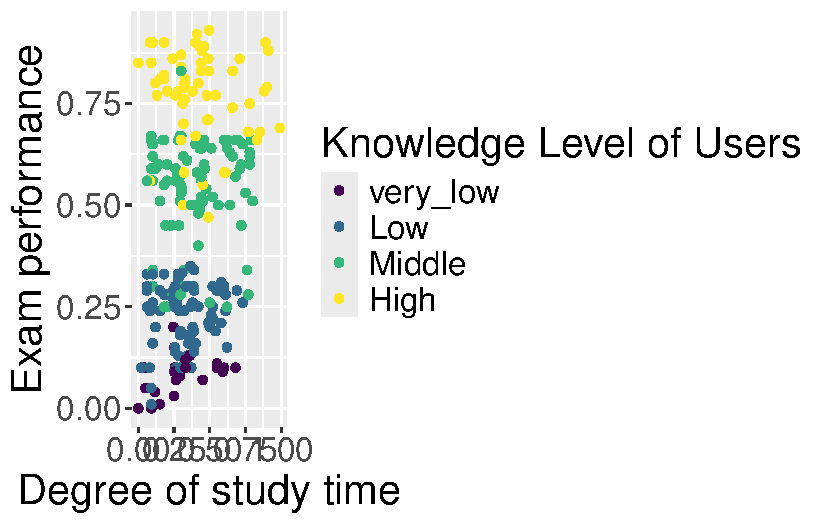
\includegraphics[keepaspectratio]{student_exam_performance_files/figure-pdf/fig-knowledge_train_summary-1.pdf}}

}

\caption{\label{fig-knowledge_train_summary}Visualization of the
distribution of Knowledge Levels based on Exam Performance and Study
Time}

\end{figure}%

\subsubsection{Main Analysis and
Results}\label{main-analysis-and-results}

In this analysis we chose to use the machine learning method of ordinal
logistic regression. Since this is a multi classification problem we
could not use simple binary logistic regression. We begin by fitting our
model and looking at the coefficients on each feature.

\begin{verbatim}
Call:
polr(formula = UNS ~ STG + PEG, data = knowledge_train_data, 
    Hess = TRUE)

Coefficients:
      Value Std. Error t value
STG  0.4481     0.8315  0.5389
PEG 23.3257     2.4173  9.6495

Intercepts:
             Value   Std. Error t value
very_low|Low  2.6636  0.5232     5.0912
Low|Middle    8.3128  0.8372     9.9291
Middle|High  16.0228  1.6559     9.6762

Residual Deviance: 232.5871 
AIC: 242.5871 
\end{verbatim}

From Table~\ref{tbl-ordinal_model} we see that exam performance has a
coefficient nearly fifty times the degree of study indicating the
feature is much more indicative of user knowledge. Now we have to see if
this model performs well on the test data

\begin{table}

\caption{\label{tbl-accuracy}Model Accuracy}

\centering{

\begin{verbatim}
[1] 0.8206897
\end{verbatim}

}

\end{table}%

Our model produces a mean accuracy of 82\% which is promising (see
Table~\ref{tbl-accuracy}). This means that really only using exam grade
as a feature allows ordinal regression to achieve high accuracy across
this complex problem.

Next we produce some visualizations to get a better sense of the data.

\begin{figure}

\centering{

\pandocbounded{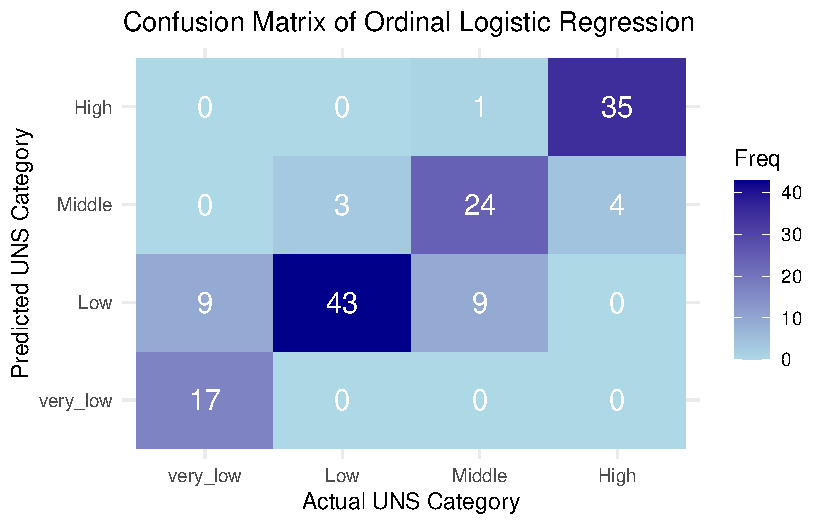
\includegraphics[keepaspectratio]{student_exam_performance_files/figure-pdf/fig-confusion_matrix-1.pdf}}

}

\caption{\label{fig-confusion_matrix}Confusion Matrix}

\end{figure}%

This confusion matrix (Figure~\ref{fig-confusion_matrix}) tells us where
our model is predicting correctly and incorrectly, as well as the
frequency to which it does that. We can see that across all possible
classes it is fairly successful with some slight confusion being
introduced when comparing the `low' and `very low' classes.

\begin{figure}

\centering{

\pandocbounded{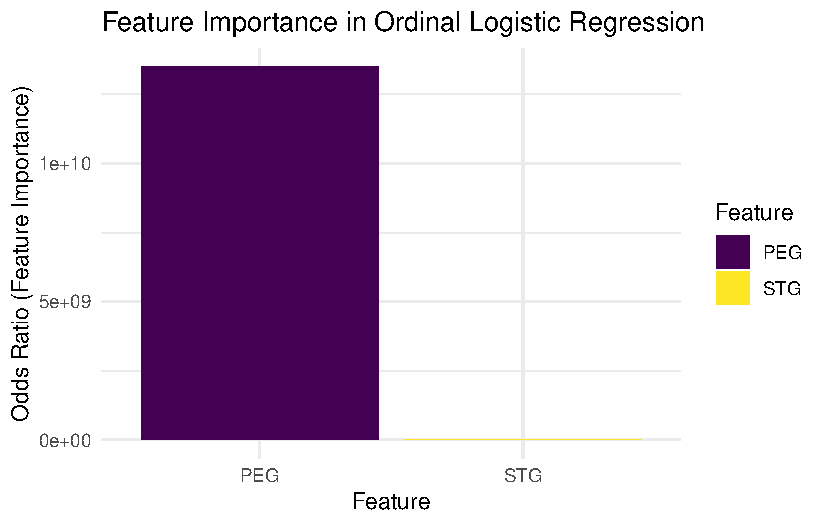
\includegraphics[keepaspectratio]{student_exam_performance_files/figure-pdf/fig-feature_inportance-1.pdf}}

}

\caption{\label{fig-feature_inportance}Feature Importance}

\end{figure}%

In Figure~\ref{fig-feature_inportance} we again look at how much
importance our model gave to each of the features we included. As seen
during fitting, exam grades is given the vast majority of the weighting
and is practically the sole predictor for our model.

\subsection{\texorpdfstring{\textbf{Discussion}}{Discussion}}\label{discussion}

During this analysis we found a model that successfully predicts user
knowledge separated by four distinct classes. We saw that when using
degree of study time and exam performance as features, exam performance
was by far the most useful predictor and dominated the model. This was
an unexpected result in terms of the magnitude of importance. We thought
that exam performance would probably be the most useful feature out of
the two, but not by so much. This shows that the exams taken where this
study was conducted is indeed a tell tale sign of user knowledge and
that time spent studying, which may increase exam performance, does not
tell us much about the users knowledge.

The impacts this study could bring about are vast. By performing a
similar result at other institutions it could be a way of confirming if
their testing procedures are representative of real life skills. This is
something every test maker hopes to achieve and could be substantiated
by a similar result as in this study.

In the future this could lead to questions regarding what else is
indicative of user knowledge other than exam performance. Are there
other indicators more important than exam performance?

We would also like to state that to improve this studies reliability we
could make some or all of the following improvements. We could use cross
validation to increase the confidence of our results, include more
features to build a more robust and accurate model, and test out other
regression techniques.

\subsection{\texorpdfstring{\textbf{Reference}}{Reference}}\label{reference}

Kahraman (2012)

\phantomsection\label{refs}
\begin{CSLReferences}{1}{0}
\bibitem[\citeproctext]{ref-kahraman2012}
Kahraman, Sagiroglu, H. T. 2012. {``The Development of Intuitive
Knowledge Classifier and the Modeling of Domain Dependent Data.''}
\url{https://www.sciencedirect.com/science/article/abs/pii/S0950705112002225?via\%3Dihub}.

\end{CSLReferences}




\end{document}
